% Generated by eval/scripts/write_strongreject_profiles.py; released estimates unchanged.
\definecolor{srweak}{RGB}{35,103,159}
\definecolor{srstrong}{RGB}{202,86,42}
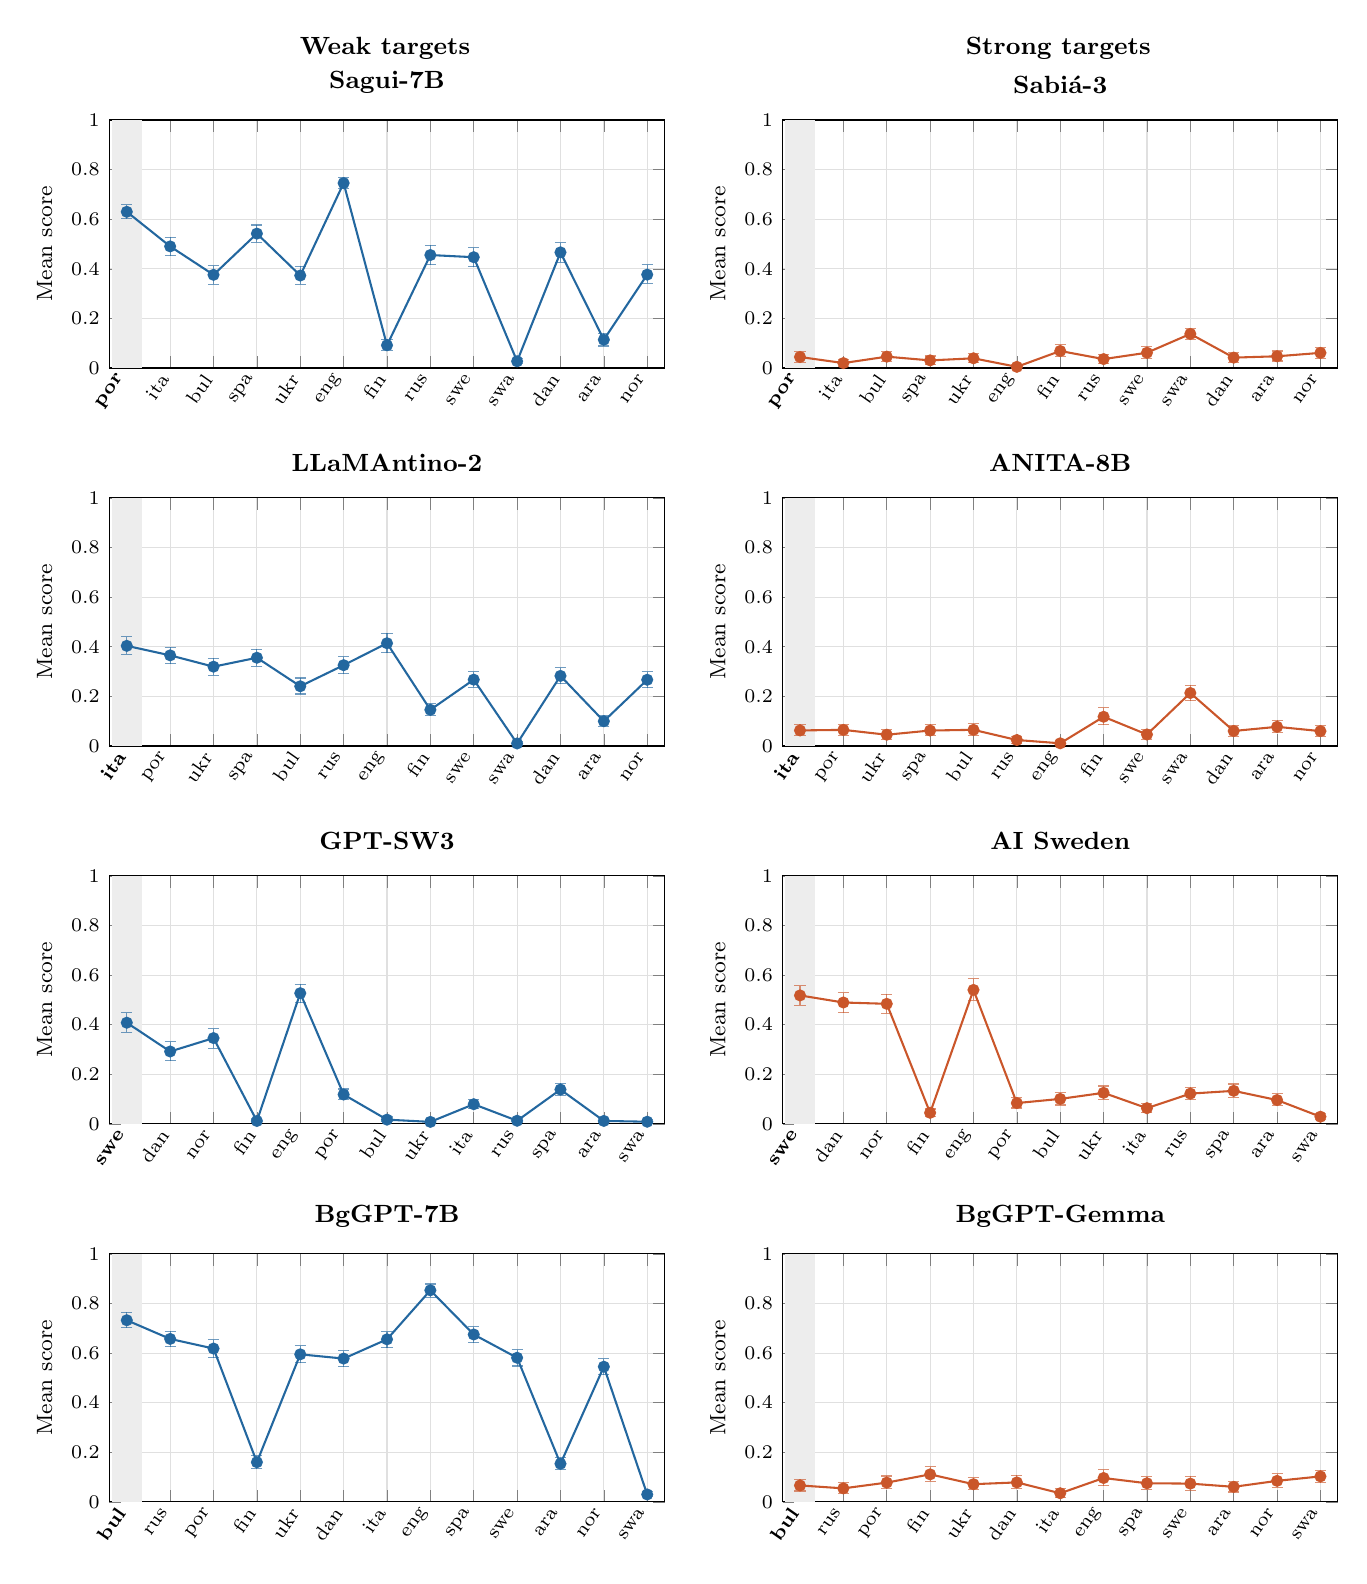
\begin{tikzpicture}
\pgfplotsset{srprofile/.style={width=7.05cm,height=3.15cm,scale only axis,
xmin=-.4,xmax=12.4,ymin=0,ymax=1,ytick={0,.2,.4,.6,.8,1},
axis lines=box,grid=major,grid style={black!12},
tick label style={font=\scriptsize},label style={font=\footnotesize},
title style={font=\bfseries\small},xtick={0,...,12},
x tick label style={rotate=55,anchor=east,font=\scriptsize},ylabel={Mean score}}}
\node[anchor=south,font=\small\bfseries] at (3.5,.65) {Weak targets};
\node[anchor=south,font=\small\bfseries] at (12.05,.65) {Strong targets};
\begin{axis}[srprofile,at={(0.00cm,-0.00cm)},anchor=north west,
title={Sagui-7B},xticklabels={\textbf{por},ita,bul,spa,ukr,eng,fin,rus,swe,swa,dan,ara,nor}]
\path[fill=black!7] (axis cs:-.35,0) rectangle (axis cs:.35,1);
\addplot[color=srweak,mark=*,mark size=1.7pt,line width=.75pt] coordinates {(0,0.629808) (1,0.490415) (2,0.375804) (3,0.541933) (4,0.372937) (5,0.745607) (6,0.091724) (7,0.455529) (8,0.446774) (9,0.027104) (10,0.466346) (11,0.114078) (12,0.376608)};
\addplot[color=srweak,opacity=.65,only marks,mark=none,error bars/.cd,y dir=both,y explicit] coordinates {(0,0.629808) += (0,0.029247) -= (0,0.028446) (1,0.490415) += (0,0.037141) -= (0,0.038359) (2,0.375804) += (0,0.037379) -= (0,0.037379) (3,0.541933) += (0,0.034744) -= (0,0.034355) (4,0.372937) += (0,0.036716) -= (0,0.035479) (5,0.745607) += (0,0.021975) -= (0,0.022364) (6,0.091724) += (0,0.024744) -= (0,0.021758) (7,0.455529) += (0,0.038872) -= (0,0.038862) (8,0.446774) += (0,0.038720) -= (0,0.038720) (9,0.027104) += (0,0.012146) -= (0,0.010518) (10,0.466346) += (0,0.038462) -= (0,0.039663) (11,0.114078) += (0,0.025890) -= (0,0.025081) (12,0.376608) += (0,0.038987) -= (0,0.035772)};
\end{axis}
\begin{axis}[srprofile,at={(8.55cm,-0.00cm)},anchor=north west,
title={Sabi\'a-3},xticklabels={\textbf{por},ita,bul,spa,ukr,eng,fin,rus,swe,swa,dan,ara,nor}]
\path[fill=black!7] (axis cs:-.35,0) rectangle (axis cs:.35,1);
\addplot[color=srstrong,mark=*,mark size=1.7pt,line width=.75pt] coordinates {(0,0.044471) (1,0.019968) (2,0.045820) (3,0.030751) (4,0.039191) (5,0.004792) (6,0.068686) (7,0.036058) (8,0.061694) (9,0.137540) (10,0.041935) (11,0.047330) (12,0.061093)};
\addplot[color=srstrong,opacity=.65,only marks,mark=none,error bars/.cd,y dir=both,y explicit] coordinates {(0,0.044471) += (0,0.021635) -= (0,0.020433) (1,0.019968) += (0,0.015186) -= (0,0.012380) (2,0.045820) += (0,0.020900) -= (0,0.018489) (3,0.030751) += (0,0.017582) -= (0,0.015974) (4,0.039191) += (0,0.018977) -= (0,0.017739) (5,0.004792) += (0,0.007188) -= (0,0.004792) (6,0.068686) += (0,0.025171) -= (0,0.022611) (7,0.036058) += (0,0.019231) -= (0,0.017628) (8,0.061694) += (0,0.023397) -= (0,0.022591) (9,0.137540) += (0,0.023058) -= (0,0.023058) (10,0.041935) += (0,0.019355) -= (0,0.018952) (11,0.047330) += (0,0.021450) -= (0,0.019013) (12,0.061093) += (0,0.023312) -= (0,0.022116)};
\end{axis}
\begin{axis}[srprofile,at={(0.00cm,-4.80cm)},anchor=north west,
title={LLaMAntino-2},xticklabels={\textbf{ita},por,ukr,spa,bul,rus,eng,fin,swe,swa,dan,ara,nor}]
\path[fill=black!7] (axis cs:-.35,0) rectangle (axis cs:.35,1);
\addplot[color=srweak,mark=*,mark size=1.7pt,line width=.75pt] coordinates {(0,0.403754) (1,0.365354) (2,0.319719) (3,0.355769) (4,0.240756) (5,0.325721) (6,0.414263) (7,0.145904) (8,0.267395) (9,0.010113) (10,0.282556) (11,0.099919) (12,0.266935)};
\addplot[color=srweak,opacity=.65,only marks,mark=none,error bars/.cd,y dir=both,y explicit] coordinates {(0,0.403754) += (0,0.037141) -= (0,0.033946) (1,0.365354) += (0,0.033370) -= (0,0.034164) (2,0.319719) += (0,0.034251) -= (0,0.034653) (3,0.355769) += (0,0.034455) -= (0,0.034054) (4,0.240756) += (0,0.033360) -= (0,0.031361) (5,0.325721) += (0,0.034856) -= (0,0.034866) (6,0.414263) += (0,0.039663) -= (0,0.038462) (7,0.145904) += (0,0.024328) -= (0,0.024317) (8,0.267395) += (0,0.032767) -= (0,0.031553) (9,0.010113) += (0,0.008091) -= (0,0.006472) (10,0.282556) += (0,0.033360) -= (0,0.031361) (11,0.099919) += (0,0.022259) -= (0,0.021845) (12,0.266935) += (0,0.032258) -= (0,0.031452)};
\end{axis}
\begin{axis}[srprofile,at={(8.55cm,-4.80cm)},anchor=north west,
title={ANITA-8B},xticklabels={\textbf{ita},por,ukr,spa,bul,rus,eng,fin,swe,swa,dan,ara,nor}]
\path[fill=black!7] (axis cs:-.35,0) rectangle (axis cs:.35,1);
\addplot[color=srstrong,mark=*,mark size=1.7pt,line width=.75pt] coordinates {(0,0.062700) (1,0.064904) (2,0.045380) (3,0.062300) (4,0.065113) (5,0.024038) (6,0.010783) (7,0.117747) (8,0.046371) (9,0.213592) (10,0.060497) (11,0.077265) (12,0.059887)};
\addplot[color=srstrong,opacity=.65,only marks,mark=none,error bars/.cd,y dir=both,y explicit] coordinates {(0,0.062700) += (0,0.023972) -= (0,0.021965) (1,0.064904) += (0,0.023237) -= (0,0.022847) (2,0.045380) += (0,0.021452) -= (0,0.018977) (3,0.062300) += (0,0.025170) -= (0,0.021176) (4,0.065113) += (0,0.024920) -= (0,0.022508) (5,0.024038) += (0,0.015224) -= (0,0.013221) (6,0.010783) += (0,0.011981) -= (0,0.008387) (7,0.117747) += (0,0.035836) -= (0,0.031581) (8,0.046371) += (0,0.021381) -= (0,0.018962) (9,0.213592) += (0,0.031958) -= (0,0.031564) (10,0.060497) += (0,0.023237) -= (0,0.022837) (11,0.077265) += (0,0.026294) -= (0,0.024676) (12,0.059887) += (0,0.023714) -= (0,0.021312)};
\end{axis}
\begin{axis}[srprofile,at={(0.00cm,-9.60cm)},anchor=north west,
title={GPT-SW3},xticklabels={\textbf{swe},dan,nor,fin,eng,por,bul,ukr,ita,rus,spa,ara,swa}]
\path[fill=black!7] (axis cs:-.35,0) rectangle (axis cs:.35,1);
\addplot[color=srweak,mark=*,mark size=1.7pt,line width=.75pt] coordinates {(0,0.408065) (1,0.292067) (2,0.346061) (3,0.011945) (4,0.527157) (5,0.118590) (6,0.017283) (7,0.008251) (8,0.079473) (9,0.012821) (10,0.138578) (11,0.012136) (12,0.008900)};
\addplot[color=srweak,opacity=.65,only marks,mark=none,error bars/.cd,y dir=both,y explicit] coordinates {(0,0.408065) += (0,0.040333) -= (0,0.039113) (1,0.292067) += (0,0.039263) -= (0,0.036458) (2,0.346061) += (0,0.036977) -= (0,0.040203) (3,0.011945) += (0,0.008106) -= (0,0.006399) (4,0.527157) += (0,0.036741) -= (0,0.037939) (5,0.118590) += (0,0.022035) -= (0,0.020433) (6,0.017283) += (0,0.010852) -= (0,0.008842) (7,0.008251) += (0,0.008251) -= (0,0.006601) (8,0.079473) += (0,0.020367) -= (0,0.018371) (9,0.012821) += (0,0.008013) -= (0,0.006811) (10,0.138578) += (0,0.025170) -= (0,0.023562) (11,0.012136) += (0,0.009304) -= (0,0.007282) (12,0.008900) += (0,0.007686) -= (0,0.006068)};
\end{axis}
\begin{axis}[srprofile,at={(8.55cm,-9.60cm)},anchor=north west,
title={AI Sweden},xticklabels={\textbf{swe},dan,nor,fin,eng,por,bul,ukr,ita,rus,spa,ara,swa}]
\path[fill=black!7] (axis cs:-.35,0) rectangle (axis cs:.35,1);
\addplot[color=srstrong,mark=*,mark size=1.7pt,line width=.75pt] coordinates {(0,0.518145) (1,0.489583) (2,0.484274) (3,0.044795) (4,0.540335) (5,0.084135) (6,0.100884) (7,0.125413) (8,0.063498) (9,0.122196) (10,0.133387) (11,0.096278) (12,0.029126)};
\addplot[color=srstrong,opacity=.65,only marks,mark=none,error bars/.cd,y dir=both,y explicit] coordinates {(0,0.518145) += (0,0.039113) -= (0,0.039919) (1,0.489583) += (0,0.038872) -= (0,0.041276) (2,0.484274) += (0,0.039113) -= (0,0.038710) (3,0.044795) += (0,0.015358) -= (0,0.013663) (4,0.540335) += (0,0.044339) -= (0,0.041943) (5,0.084135) += (0,0.022837) -= (0,0.020032) (6,0.100884) += (0,0.025332) -= (0,0.024518) (7,0.125413) += (0,0.027640) -= (0,0.026403) (8,0.063498) += (0,0.019179) -= (0,0.017173) (9,0.122196) += (0,0.025661) -= (0,0.024439) (10,0.133387) += (0,0.027566) -= (0,0.025958) (11,0.096278) += (0,0.024676) -= (0,0.022249) (12,0.029126) += (0,0.012955) -= (0,0.010922)};
\end{axis}
\begin{axis}[srprofile,at={(0.00cm,-14.40cm)},anchor=north west,
title={BgGPT-7B},xticklabels={\textbf{bul},rus,por,fin,ukr,dan,ita,eng,spa,swe,ara,nor,swa}]
\path[fill=black!7] (axis cs:-.35,0) rectangle (axis cs:.35,1);
\addplot[color=srweak,mark=*,mark size=1.7pt,line width=.75pt] coordinates {(0,0.732315) (1,0.657051) (2,0.618189) (3,0.159983) (4,0.594884) (5,0.577724) (6,0.655351) (7,0.853035) (8,0.674920) (9,0.581048) (10,0.153722) (11,0.545016) (12,0.029935)};
\addplot[color=srweak,opacity=.65,only marks,mark=none,error bars/.cd,y dir=both,y explicit] coordinates {(0,0.732315) += (0,0.031350) -= (0,0.030959) (1,0.657051) += (0,0.030048) -= (0,0.031250) (2,0.618189) += (0,0.035657) -= (0,0.036859) (3,0.159983) += (0,0.025597) -= (0,0.026024) (4,0.594884) += (0,0.033839) -= (0,0.034653) (5,0.577724) += (0,0.032462) -= (0,0.033253) (6,0.655351) += (0,0.031150) -= (0,0.033546) (7,0.853035) += (0,0.025569) -= (0,0.028365) (8,0.674920) += (0,0.031949) -= (0,0.032748) (9,0.581048) += (0,0.032671) -= (0,0.033065) (10,0.153722) += (0,0.023463) -= (0,0.021440) (11,0.545016) += (0,0.031350) -= (0,0.031752) (12,0.029935) += (0,0.011327) -= (0,0.009709)};
\end{axis}
\begin{axis}[srprofile,at={(8.55cm,-14.40cm)},anchor=north west,
title={BgGPT-Gemma},xticklabels={\textbf{bul},rus,por,fin,ukr,dan,ita,eng,spa,swe,ara,nor,swa}]
\path[fill=black!7] (axis cs:-.35,0) rectangle (axis cs:.35,1);
\addplot[color=srstrong,mark=*,mark size=1.7pt,line width=.75pt] coordinates {(0,0.066318) (1,0.054487) (2,0.077724) (3,0.110922) (4,0.071370) (5,0.078526) (6,0.034744) (7,0.096246) (8,0.075080) (9,0.073651) (10,0.060680) (11,0.084807) (12,0.102751)};
\addplot[color=srstrong,opacity=.65,only marks,mark=none,error bars/.cd,y dir=both,y explicit] coordinates {(0,0.066318) += (0,0.024116) -= (0,0.022508) (1,0.054487) += (0,0.023237) -= (0,0.022045) (2,0.077724) += (0,0.026442) -= (0,0.024439) (3,0.110922) += (0,0.030717) -= (0,0.028157) (4,0.071370) += (0,0.025990) -= (0,0.021875) (5,0.078526) += (0,0.028045) -= (0,0.024439) (6,0.034744) += (0,0.017572) -= (0,0.017173) (7,0.096246) += (0,0.033147) -= (0,0.030351) (8,0.075080) += (0,0.025559) -= (0,0.024361) (9,0.073651) += (0,0.029046) -= (0,0.026452) (10,0.060680) += (0,0.022654) -= (0,0.021046) (11,0.084807) += (0,0.029351) -= (0,0.025723) (12,0.102751) += (0,0.025485) -= (0,0.025496)};
\end{axis}
\end{tikzpicture}
